To setup the hardware, one can either:
\begin{itemize}
	\item Build the design himself as described in the previous sections
	\item Use the binaries provided in \emph{<repo>/build}
\end{itemize}
An SD card of at least $4GB$ needs to be formatted as FAT32 and contain the
following files:
\begin{itemize}
	\item \emph{BOOT.BIN}: Contains the \gls{fsbl}, u-boot and the bistream
		for the \gls{pl}
	\item \emph{zImage}: The linux kernel
	\item \emph{root.img}: The Android Operating System
	\item \emph{devicetree.dtb}: The compiled devicetree
	\item \emph{blake2b.ko}: The kernel module for the hashing device
	\item \emph{image\_filter.ko}: The kernel module for the image filters
	\item \emph{ramdisk8M.image.gz}: The ramdisk
	\item \emph{startup.sh}: The script that loads the kernel modules
	\item \emph{startup\_android.sh}: The script that starts Android. If this
		file is missing the boot process will only boot the linux kernel
\end{itemize}
The jumpers on the ZedBoard must be set up as follows:

\begin{center}
	\begin{tabular}{lc}
		JP1 & open\\
		JP2 & short\\
		JP3 & short\\
		JP4 & (open / not populated)\\
		JP5 & (open / not populated)\\
		JP6 & short\\
		JP7 & GND\\
		JP8 & GND\\
		JP9 & 3V3\\
		JP10 & 3V3\\
		JP11 & GND\\
		JP12 & open\\
		JP13 & open\\
		JP18 & 1V8\\
	\end{tabular}
\end{center}
A USB hub can be connected at the \gls{otg} connector.
This can then host a USB Keyboard and the USB touchscreen connector
A \gls{uart} interface is available at the \gls{uart} USB port.
The SD card needs to be inserted into the SD card slot (on the backside of
the ZedBoard, under the FMC connector).
An Ethernet cable can be connected to the Ethernet port.
This can be seen in \Cref{fig:zedboardsetup}.

\begin{figure}[h]
\centering
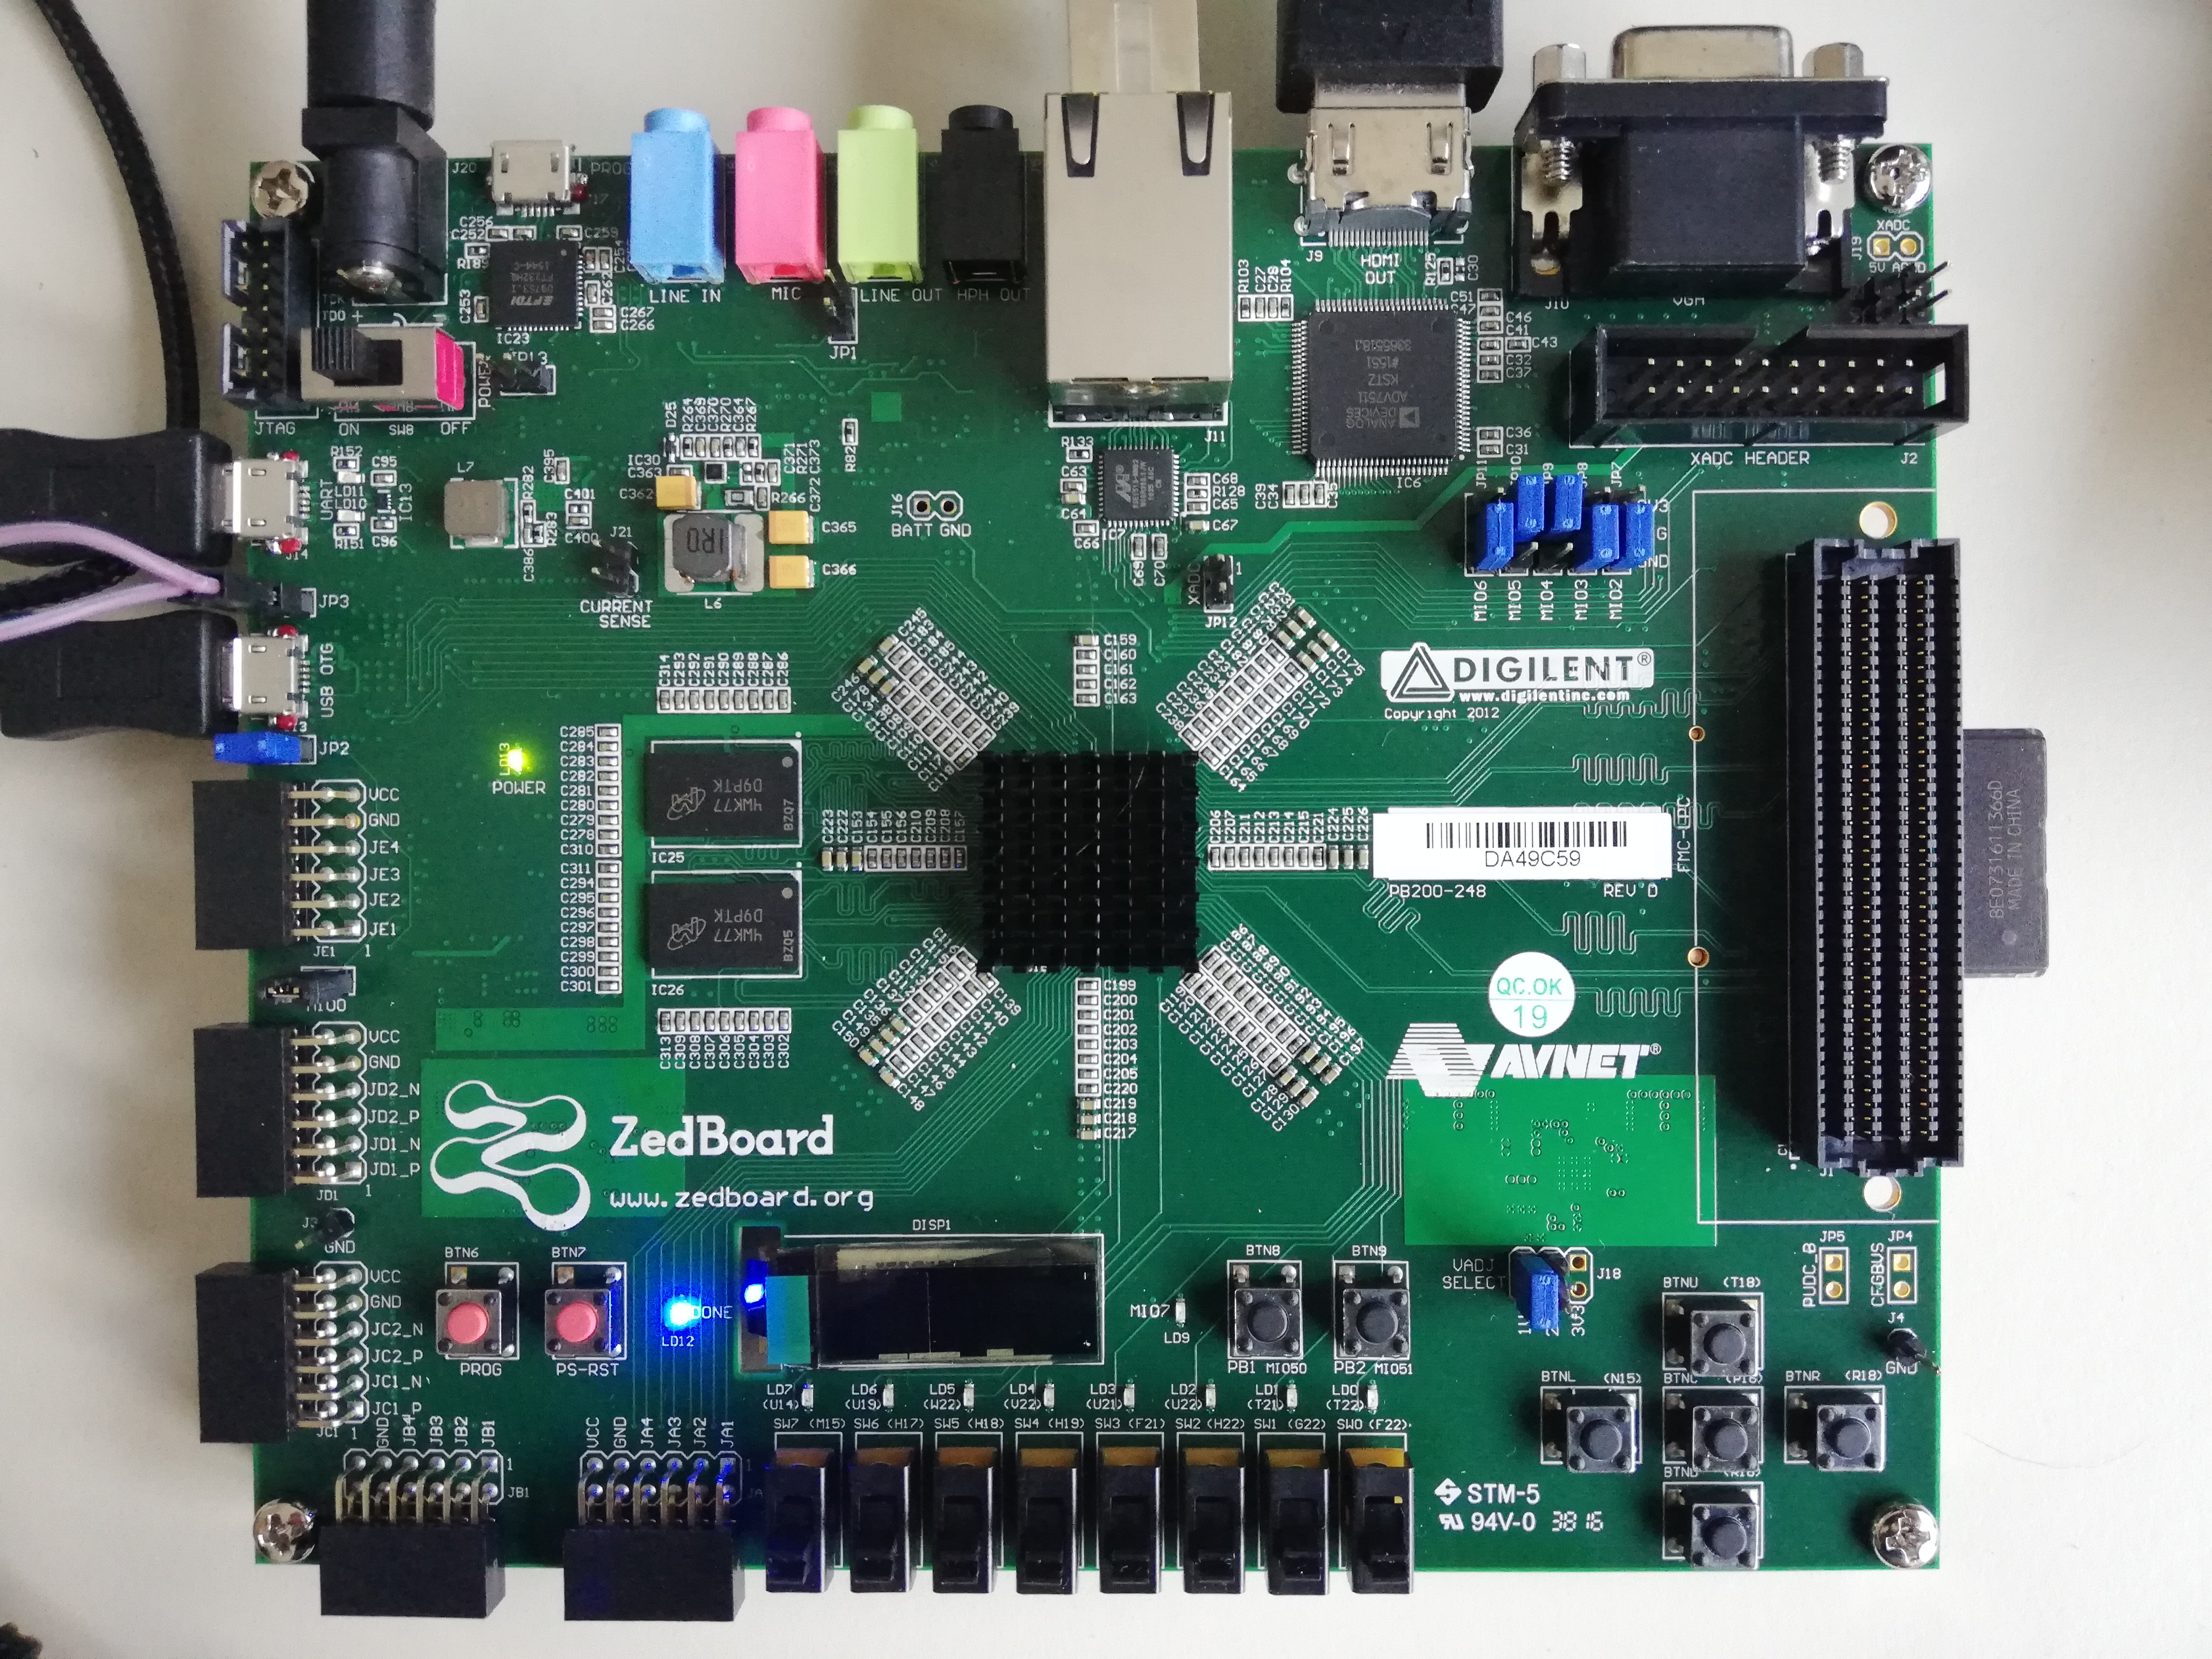
\includegraphics[width=1\textwidth]{sections/methodology/zedboardsetup}
\caption{\label{fig:zedboardsetup} ZedBoard setup}
\end{figure}

Once everything is set up, the power switch can be switched to the \emph{ON}
position and Android will boot.
After boot, Android will present itself on the display and show the launcher
as seen in \Cref{fig:androiddisplay}.

\emph{NOTE:} The screen must be connected before boot, otherwise the Android
\gls{gui} will not show.

\begin{figure}[h]
\centering
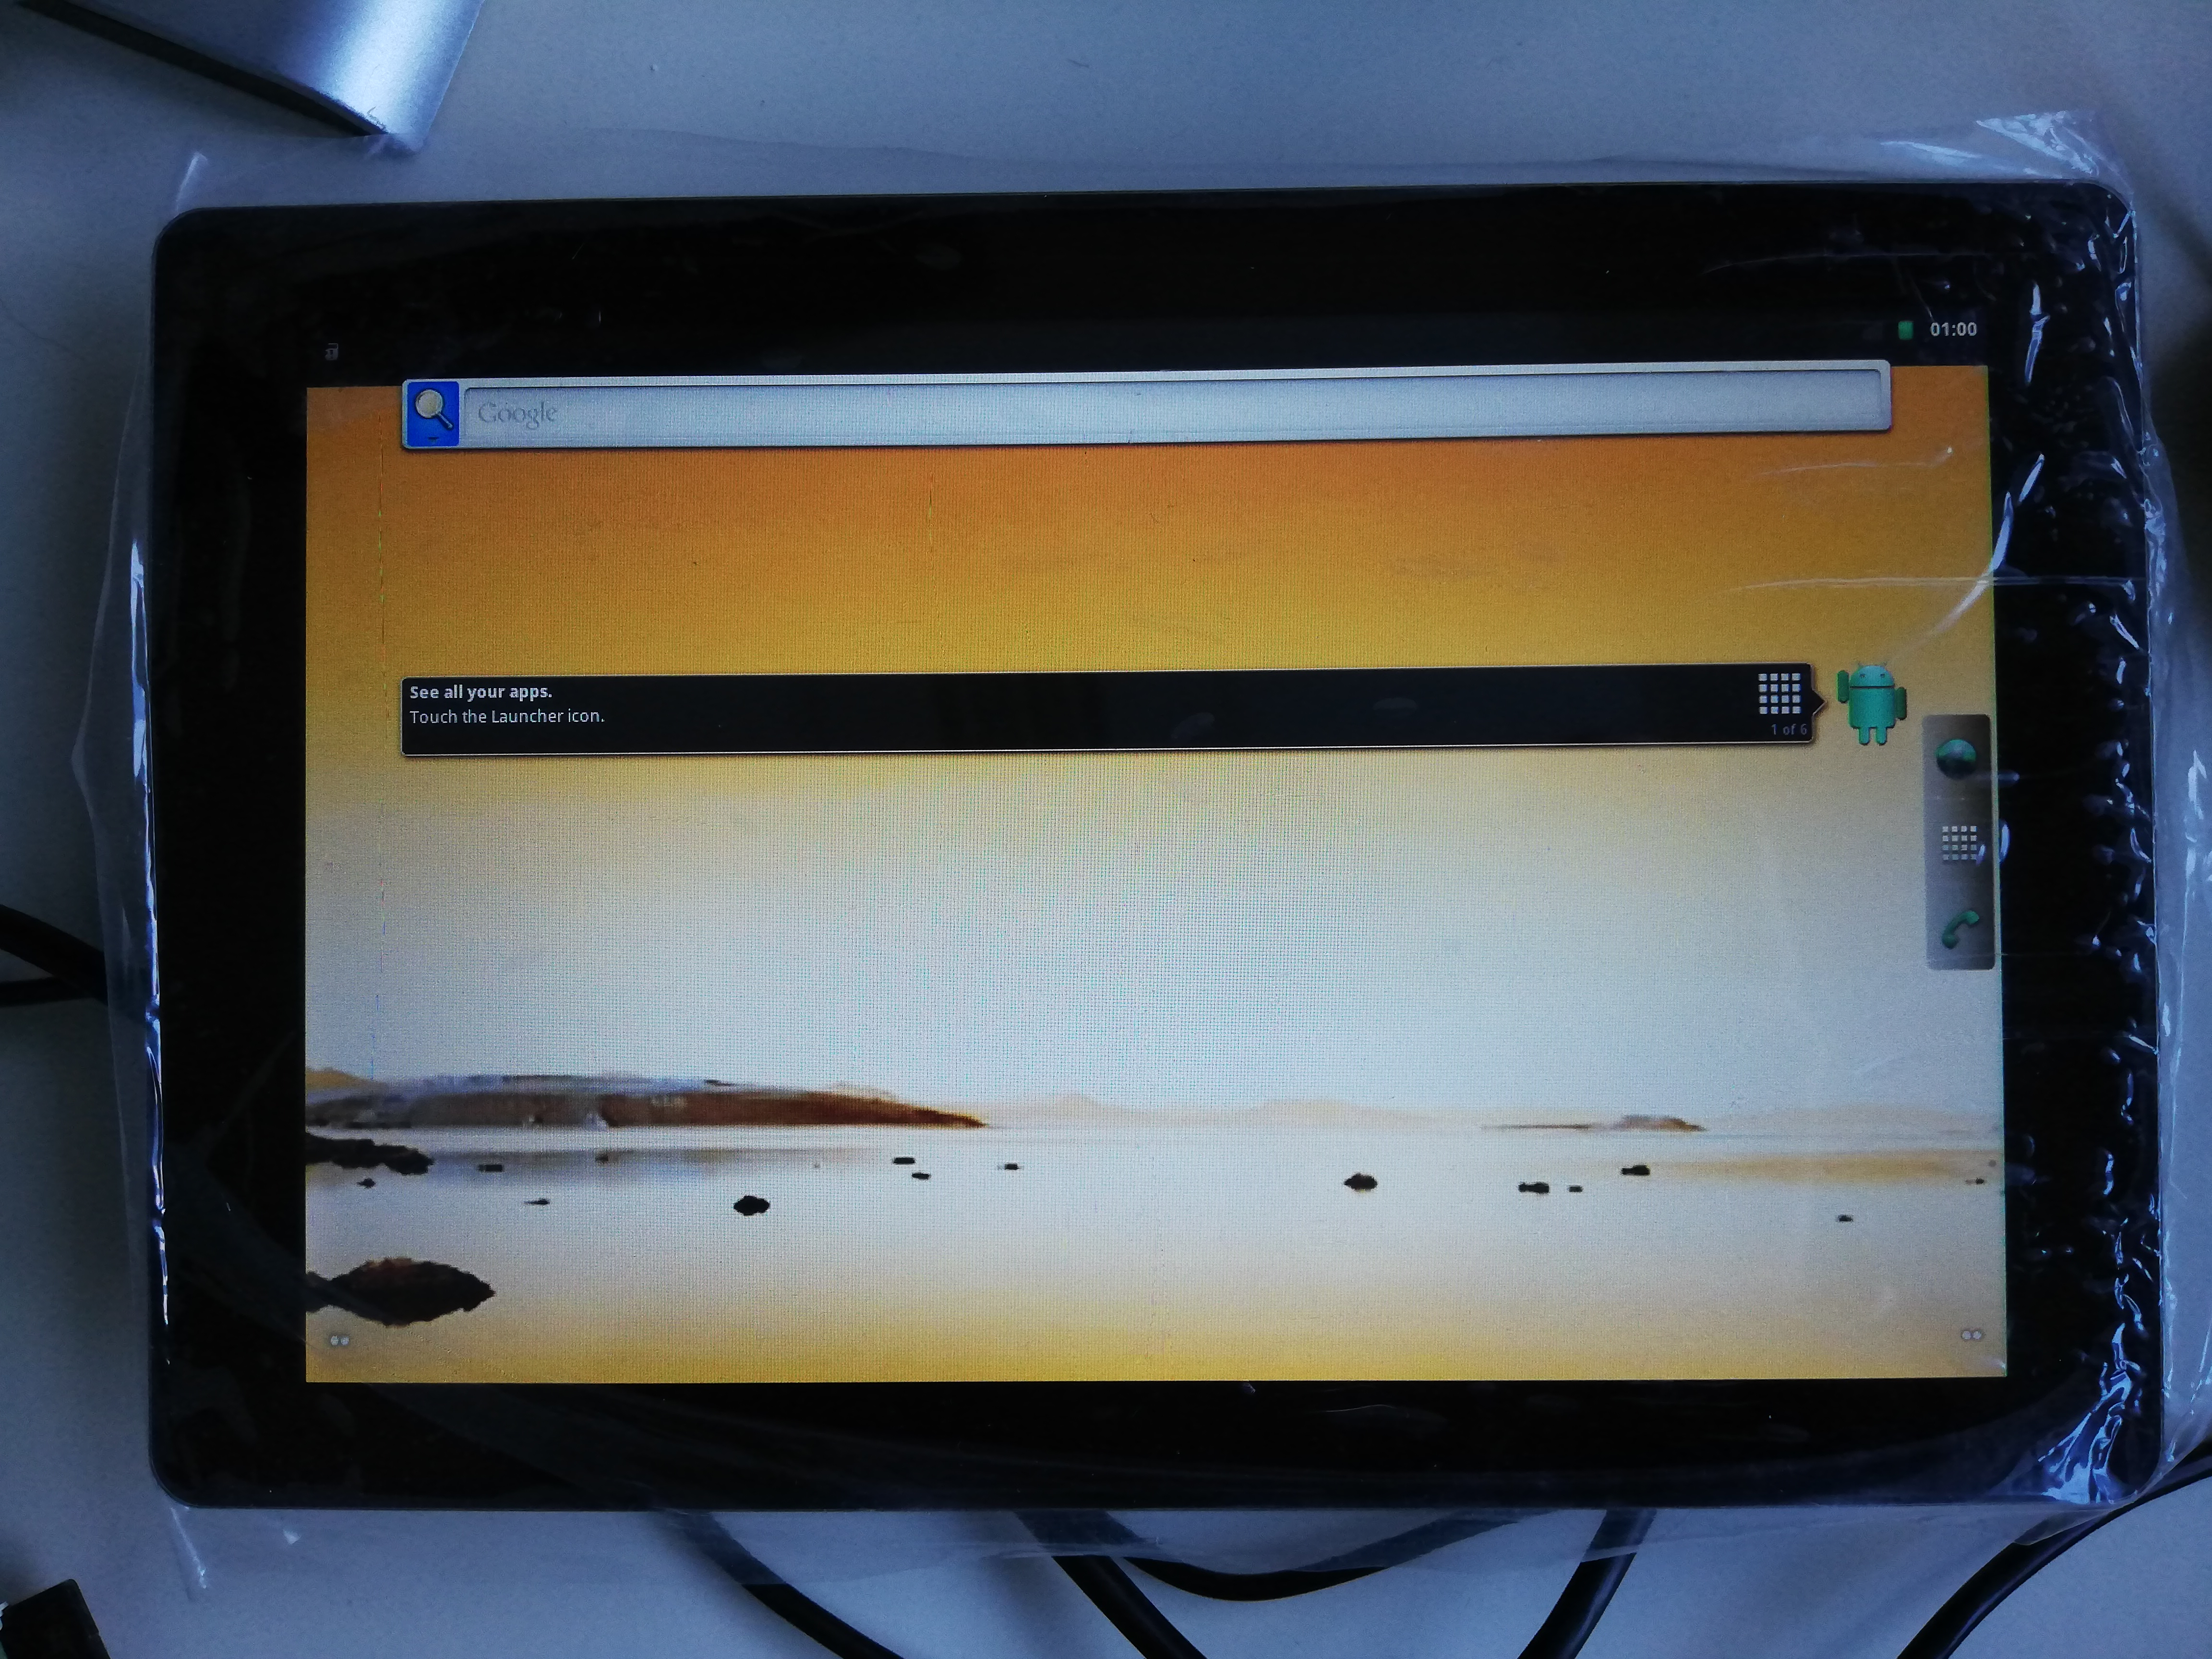
\includegraphics[width=1\textwidth]{sections/methodology/androiddisplay}
\caption{\label{fig:androiddisplay} Android launcher on the ZedBoard display}
\end{figure}
